\subsection{Regularized logistic regression for whole-brain pattern classification}
\subsubsection{Concepts}
The limitations of the searchlight method arise from the relationship between a searchlight's field of view and the anatomical distribution of the underlying signal. A small searchlight provides better localization but is more likely to exclude signal-carrying units; a large searchlight is more likely to include the signal-carrying units but provides less information about where the signal really is. 

An alternative approach that avoids this tradeoff is to train a pattern classifier on the whole dataset simultaneously. While many classification algorithms exist, we focus here on variants of logistic regression because they are easily interpretable, powerful, and draw upon intuitions formed through experience with linear regression. A regression model is composed of a set of weights $\beta_X$, one for each predictor variable $x$ plus an additional intercept term, tuned to make accurate predictions about a response variable $y$. In logistic multivariate pattern classification, the predictor variables are the voxels, and the response is a binary variable that codes class or condition label. For instance, in a contrast of conditions A and B, A events are labeled with $y=1$ and B events are labeled with $y=0$. To generate a prediction for a given item, the logistic regression model takes the weighted sum of the estimated response over voxels and passes it through a squashing function bounded at 0 and 1:

\begin{align}
f(z) = \frac{e^z}{1+e^{z}}
\label{eq.logisticloss}
\end{align}

Where $z = \beta_0 + \beta_1X_{i 1} + \beta_2X_{i 2} + \dots +  \beta_nX_{i n} + \epsilon_{i}$---the model's linear response to a particular pattern of activity. Thus, $f(z)$ is a transformation of the weighted sum of predictor values expressing the probability that $y=1$ given the pattern of activity for the $i^{th}$ item. Fitting a logistic regression model involves finding coefficients that minimize the discrepancy between the true labels in $y \in{\{0,1\}}$ and the probabilities assigned by the model. This is typically measured by the logistic loss:

\begin{align}
%\argmin_\beta \sum^{n}_{i=1}{\left(y_i-f\left( X_i\beta + \beta_0\right) \right)^2}
\argmin_\beta \sum^{n}_{i=1}{\log(1 + e^{\bar{-y_i} X_i\beta})}
\label{eq.logisticopt}
\end{align}

...where $\bar{y_i}$ is -1 when $y_i=0$ and +1 when $y_i=1$. This loss is minimized when the sign of the model's linear response $X_i\beta$ is positive for items labeled $y=1$ and negative for items labeled $y=0$.

As noted previously, the problem is that there are infinite possible solutions to the minimization when there are more predictors than items. One needs a way of deciding which among these is most likely to uncover the real signal. {\em Regularized} regression provides one way of doing this. Such approaches seek to jointly minimize the prediction error plus an additional cost, itself a function of the coefficients:

\begin{align}
\argmin_\beta \sum^{n}_{i=1}{\log(1 + e^{\bar{-y_i} X_i\beta})} + \lambda h(\beta)
\label{eq.regularized}
\end{align}

The additional penalty or {\em regularizer} represented by $h(\beta)$ prioritizes some model solutions over others, and in this way embodies a hypothesis about the nature of the true underlying signal. The constant $\lambda$ is a free parameter that controls the degree to which the two terms (prediction error versus minimization of the regularizer) should be weighted in the joint optimization.

We here consider two varieties of regularized logistic regression recently employed in the fMRI literature: {\em LASSO}\cite{rish_sparse_2012} and {\em ridge regression} \cite{riggall_relationship_2012}. Though superficially similar, the two methods embody different implicit assumptions about the nature of the underlying signal and so yield quite different results. In LASSO, the regularizer is the sum of the absolute values of the model coefficients:

\begin{align}
h(\beta) = \sum^m_{j=1} |\beta_j|
\label{eq.lasso}
\end{align}

For ridge regression, the penalty is the sum of their squared values:

\begin{align}
h(\beta) = \sum^m_{j=1}\beta_j^2
\label{eq.ridge}
\end{align}

In both cases, the optimization is convex: for a given value of $\lambda$, there exists a unique set of coefficients that minimize the cost and that can be efficiently discovered by gradient descent. Yet the different penalties lead to quite different solutions. To understand why, it is useful to consider how they treat sets of predictors that covary together with one another. Imagine 4 voxels whose responses across items are perfectly correlated, and suppose their activations are useful in predicting the condition label. In this scenario, there are many different ways of placing weights over the 4 voxels that will all have the same effect on the classifier output. For instance, placing a weight of 1 on each voxel will have exactly the same effect as placing a weight of 4 on one voxel and a weight of 0 on the other three. Because the voxel activations are perfectly correlated, and the classifier operates on a weighted sum over voxel activations, these different weight configurations have the same effect on the model output and hence on the prediction error. The regularization penalty, however, should prefer some weight configurations over others.

If the data really are perfectly correlated, the LASSO penalty won't be any help: the sum of the absolute value of the coefficients is the same for models that place a 1 on each unit versus models that put a 4 on one unit and zeroes on the rest. If we imagine, however, that all measurements are subject to some independent noise, the scenario is a bit different. In this case, one of the 4 units will, just by chance, covary slightly better with the category labels. In this case, the classifier can do a slightly better job of minimizing the error term by loading up all of the weight on this single voxel. Thus the joint optimization will lead to a solution where just one (or perhaps a few) of the redundant voxels are selected. Ridge regression behaves very differently. Here the penalty scales exponentially as weights increase on a single voxel, but only linearly as weights are added across voxels. Thus the penalty is minimized by placing small weights on many voxels. In the preceding example, placing a weight of 4 on one unit and 0 on the remaining 3 leads to a total penalty of 16 over the 4 units. Placing a weight of 1 on each unit, in contrast, leads to a penalty of 4. Ridge regression thus prefers solutions where small weights are "spread out" over redundant predictors. In fact, as the weight approaches zero, the ridge penalty becomes vanishingly small, so with a finite number of training examples, ridge regression will always place a tiny weight on every predictor. In real data, of course, voxel states are never perfectly correlated nor perfectly informative about the condition label, so the behaviors of the two approaches are less easy to intuit. In general, however, it is useful to think of LASSO as minimizing prediction error with the {\em fewest} possible predictors (ie, as many zero coefficients as possible), while ridge regression can be viewed as "spreading" small weights over all predictors exhibiting any systematic relationship with the category labels, without care for the number of predictors. 

What assumptions do these approaches then bring about the nature of the underlying representation? Let's first consider the univariate assumptions: 

\begin{enumerate}
\item Localization within individuals: Both methods operate on all voxels at once and are blind to anatomical relations among voxels, so no localization is assumed.

\item Consistency of coding within individual representations: Both methods allow for the placement of any weight on any voxel so there is no assumption that information is encoded in the same way across representational elements.

\item Localization across individuals: These analyses are intrinsically single-subject analyses: each classifier is trained and tested on each participant individually, and each participant yields a unique solution. Thus no localization across individuals is assumed

\item Consistency of coding across individuals: Because the analyses are applied separately to individual subjects, no consistency of coding across individuals is assumed.

\item Independence of representational units: Classifier outputs operate on patterns of activation elicited over the whole brain, so the approach does not assume that activations of individual voxels, or even sets of voxels within particular cortical regions, can be interpreted independently.
\end{enumerate}

These approaches thus relax {\em all} of the univariate assumptions (and likewise the assumptions of the searchlight approach). This does not mean that they are assumption-free: to the contrary, each approach entails additional assumptions about the {\em sparsity} and the {\em redundancy} of the underlying signal:

\begin{enumerate}
\setcounter{enumi}{5}
\item Sparsity: LASSO assumes the signal to be {\em sparse}, in that only a small proportion of voxels are involved in coding the information of interest. In this case, the best approach to finding true signal is to minimize prediction error using the smallest number of predictors possible. Ridge regression makes no sparsity assumption.

\item Redundancy: Ridge regression assumes that the signal is highly redundant, so that many voxels express essentially the same information. In this case the best approach to finding true signal is to minimize prediction error using distributions of weights that are as close to zero as possible, so that all informative predictors are included in the solution. LASSO assumes that the underlying signal is {\em not} highly redundant, so that different predictors carry different information.
\end{enumerate}

With these assumptions, what signal does LASSO and ridge regression detect in the model?

\subsubsection{Implementation}
Logistic LASSO and ridge regression were conducted using glmnet (Friedman, Hastie, \& Tibshirani, 2010) in \matlab (2013a). Both methods have a free parameter $\lambda$ that controls the importance of the regularization penalty relative to the prediction error, leading to greater sparsity in LASSO and more severe weight shrinkage in ridge regression. The analysis thus proceeded in two steps: one to estimate a useful $\lambda$ for each subject, and a second to fit a model at the estimated $\lambda$ and evaluate it on a hold-out set. The data for each model subject was first divided into 6 equal parts, each containing the same number of category A and B items. One part was set aside and the remaining 5 were passed to a function that conducted a 5-fold cross validation accuracy test at 100 values of $\lambda$. The function returns the $\lambda$ producing the highest cross-validation accuracy, which is subsequently used to fit a model to all 5 parts of the data. The resulting model was then assessed on the original hold-out set (the 6th part). This procedure was carried out separately for all 10 model subjects, in both localized and anatomically dispersed model variants, for both LASSO and ridge regression. For each model subject, each method returns a vector of coefficients that indicates how the classifier interprets each unit's activation in generating a predicted class label. To understand which units contribute to the representation of interest and how these units encode information, the coefficients must be interpreted. A key difference between methods lies in the ease of interpretation. We will therefore consider results from the two methods separately, before contrasting them.

\subsubsection{Results for LASSO}

\begin{center}
\textbf{---Figure \ref{fig.lasso} about here---}
\end{center}

\begin{figure}
\centering
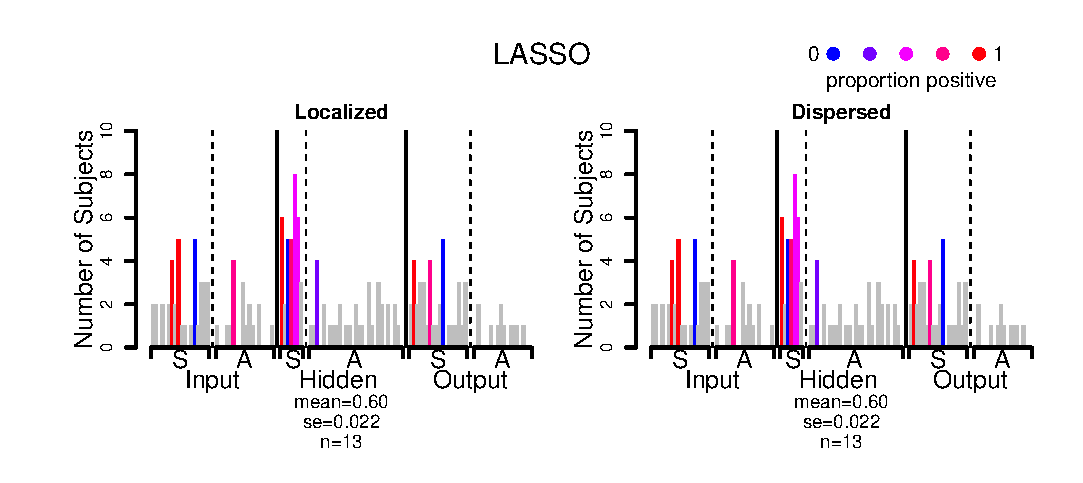
\includegraphics[width=0.95\textwidth]{figures/lasso_only.eps}
\caption{The results from the LASSO analysis. The height of each bar indicates the number of times each unit was selected, that is, given a non-zero weight over subjects. Colored bars were selected more often than expected by chance given the overall rate of unit selection. The blueness or redness of the bar conveys the frequency with which each unit was assigned a positive weight over subjects. Positive weights mean that activation at that unit will push the model towards labeling the current item as belonging to domain A. Mean and se indicate the mean and standard error of the classifier accuracy, respectively; n indicates the number of units selected more often than chance across model subjects.}
\label{fig.lasso} 
\end{figure}

For LASSO, interpretation of the classifier coefficients is straightforward: the method places zero weights on as many predictors as possible, so any unit receiving a non-zero weight can be viewed as having been ``selected'' by the classifier as important. If the classifier shows above-chance cross-validation accuracy, we can be certain that it has successfully identified signal-carrying units. In contrast to the preceding methods, there is no statistical test performed on a null hypothesis at each unit. Instead, any selected unit in a given model individual can be viewed as ``significant'' for the representation because, if it could be discarded without affecting classifier performance, LASSO would have done so. In this sense, for each subject, the method can be viewed as finding the {\em smallest sufficient set} for classification. The central questions then are (1) how well does the selected set pick out the signal-carrying voxels in I/O and hidden layers, (2) do the classifier weights indicate differences in how information is encoded for different voxel sets and (3) do the results differ for localized versus dispersed model variants?

Figure \ref{fig.lasso} shows how often LASSO selected each unit across the 10 model subjects for localized versus dispersed cases. To get a sense of which units were selected more often than expected by chance, we took the overall proportion of units selected across subjects as a base probability for conducting a binomial test at each unit. Colored bars indicate units that were selected more frequently than expected if LASSO was choosing at random with this base rate, without correction for multiple comparisons. From this plot, the approach does a fairly good job of identifying the SH units, reliably tagging 5 of the 7 units (71\%). The approach did less well discovering the systematic I/O units, reliably identifying only 6/36 (17\%). This difference reflects the fidelity of the representations coded across different unit sets: as already noted, the 7 SH units encode the cleanest representation of the domain distinction, and so are more likely to be included in the smallest sufficient set for any individual. Also, note that the results are identical for localized versus dispersed cases. Since LASSO is conducted separately for each individual and is blind to anatomical structure, the results are literally identical regardless of how the units are spatially arranged.

This summary plot is misleading in one sense, however, since it applies an aggregate statistical test across model individuals to assess which units are reliably discovered. Such a test would not be possible with real data, since it would not be clear which voxels should be ``lined up'' across subjects to compute the binomial probabilities. The virtue of LASSO (and ridge regression) is that they are essentially single-subject analyses, and so are freed from assumptions about consistency in location and coding across individuals. What we really wish to know is how accurately the solution picks out the units of interest {\em for each individual model}. For every model individual, from the binary classification of selected versus unselected units, we can compute two numbers that jointly describe how well the solution identifies the important units. Specifically, we compute the {\em hit rate}, which is the proportion of actual signal-carrying units identified by the algorithm, and the {\em precision}, which indicates what proportion of the selected units are true signal-carrying voxels. Moreover, these figures can be tallied for just the I/O units, just the hidden units, and for the whole network, to provide an indication of how well the method singles out informative units in these different sets. 

\begin{center}
\textbf{---Figure \ref{fig.precision} about here---}
\end{center}

\begin{figure}
\centering
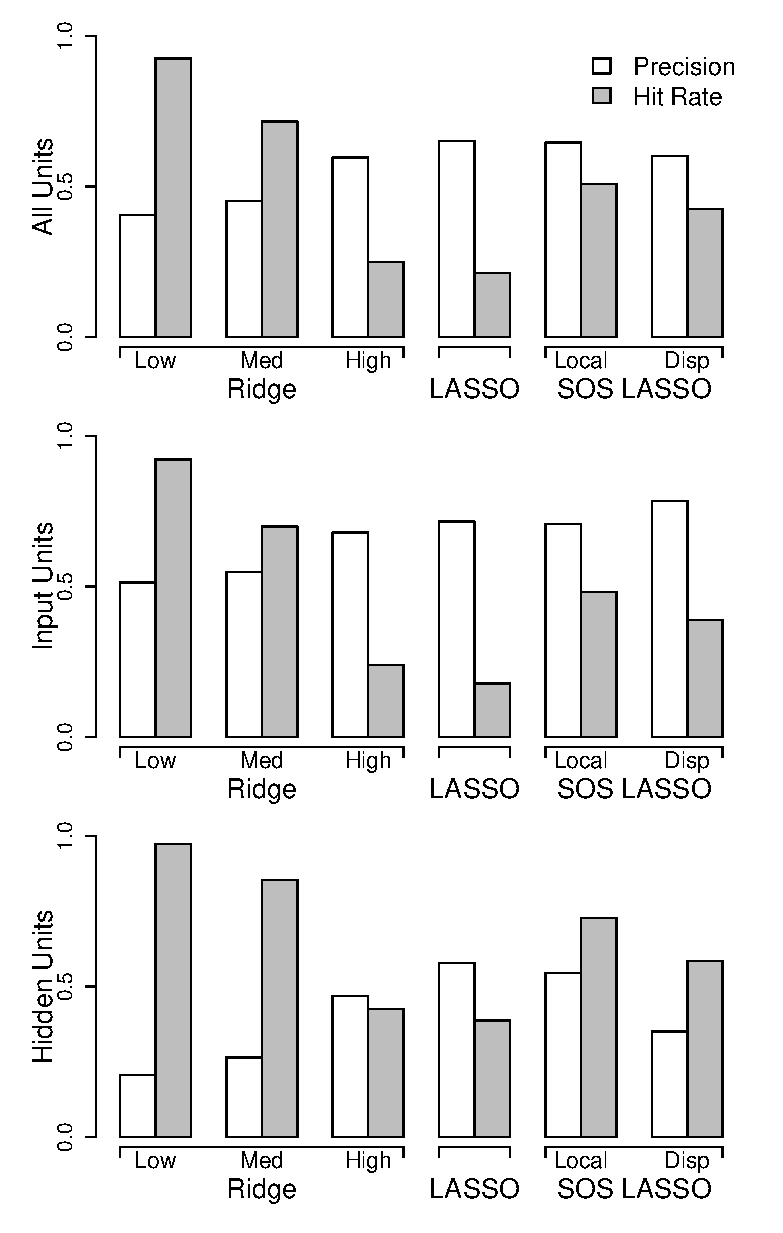
\includegraphics[width=0.6\textwidth]{figures/precision_plot.eps}
\caption{\label{fig.precision} Hit rate and precision for different multivariate methods, computed across the whole network (top), the I/O units only (middle), and the hidden units only (bottom).}
\end{figure}

Figure \ref{fig.precision} shows the mean of these figures across model individuals for LASSO (and other methods). The general pattern is clear: precision is relatively high, indicating that most of the units LASSO identifies are indeed signal-carrying units. LASSO is sub-optimal, however, in the hit rate: for the hidden layer, about half the important units are missed, while the great majority of signal-carrying units are missed in the I/O layer. Thus if LASSO selects a unit, one can have confidence that it does carry useful information, but one cannot have confidence that it has discovered all the useful elements.

Finally, we can ask how well LASSO uncovers differences in the representational code. The red-blue spectrum of the colored bars in Figure \ref{fig.lasso} indicates the frequency with which each unit receives a positive weight across model subjects. Red and blue colors indicate that a unit's activation receives the same interpretation across model subjects, while shades in between indicate that the interpretation varies. The Figure shows that, where LASSO does identify systematic I/O units, it also reveals the correct code: all units are red or blue. There are so few units identified, however, it is difficult to ``see'' the systematic layout of these responses. In the SH layer, LASSO correctly indicates that code can vary across individuals for some units, though it also appears to show consistent category-selective responses for some units. These differences arise because LASSO does not succeed in selecting all SH units in every model individual. Instead, each unit is identified in about half of the individuals. When the algorithm selects a unit in a small set of participants, all of whom happen to have acquired the same code, the selected unit appears to show a selective code.

In sum, LASSO yields the following answers to the four questions:
\begin{enumerate}
\item {\bf Does the method reliably identify the systematic I/O units?} No. The I/O units it identifies tend to be systematic, but many such units are missed.
\item {\bf Does the method reliably identify the systematic hidden units?} It does so moderately well: each unit is selected in about half the subjects, while arbitrary units are rarely selected.
\item {\bf Does the method indicate how the information of interest is coded across identified units?} It does so quite well for identified units, though few I/O units are identified and each SH unit is only identified in about half of the individuals.
\item {\bf Do method results depend on anatomical localization of signal-carrying units?} No. The method is applied separately to each individual and is blind to anatomical structure so the results for each individual are identical regardless of the anatomical arrangement of the network.
\end{enumerate}

\subsubsection{Results for ridge regression}

\begin{center}
\textbf{---Figure \ref{fig.ridge} about here---}
\end{center}

\begin{figure}
\centering
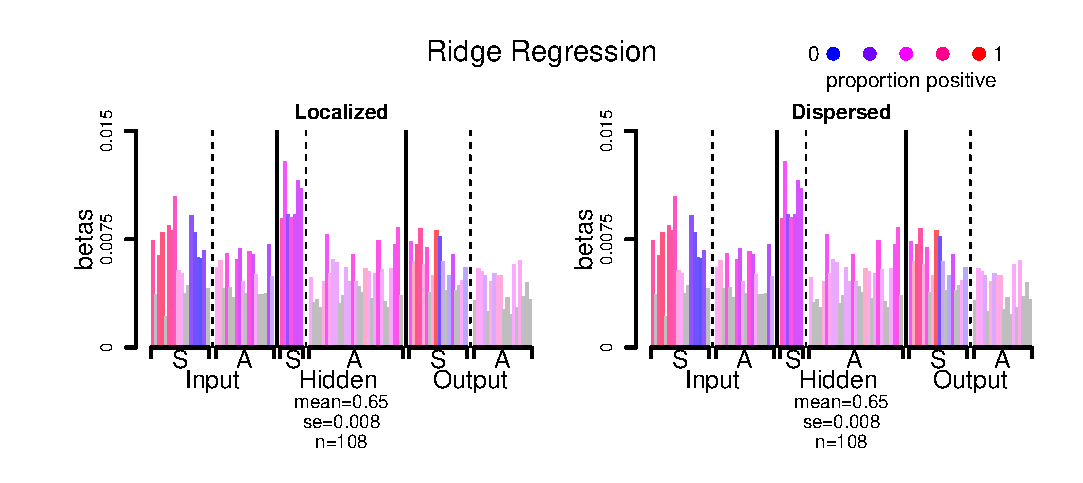
\includegraphics[width=0.95\textwidth]{figures/ridge_only.eps}
\caption{\label{fig.ridge} The results from the ridge regression analysis. Height of each bar indicates the mean across model subjects of the absolute value of the weight placed on each unit by the classifier. Bar hue indicates the frequency with which each unit received a positive weight across model subjects. Bar saturation indicates which units would count as "selected" under three different policies, based on weight magnitude. Bright bars are in the top third of the distribution, pale bars are in the middle third, and gray bars are in the bottom third. Mean and se indicate the mean and standard error of the classifier accuracy, respectively; n indicates the mean number of units with non-zero weights across model subjects.}
\end{figure}

The ridge regression classifier showed marginally better cross-validation accuracy (0.65 compared to 0.6 for LASSO), but with a very different distribution of weights. In fact, ridge regression placed a non-zero weight on every unit--effectively using the whole pattern of activation across all units in the network. Consequently it is difficult to know which predictors are playing an important role in the classifier behavior and which are not. Weight size (i.e., absolute value of a weight) provides one indicator of predictor importance, since the regularization penalty tries to keep weights as close to zero as possible. Any predictor receiving a weight that deviates strongly from zero must, therefore, be important for reducing prediction error. But this relationship is not perfectly transparent. Consider the case where a single unit carries important information for classifying one subset of items, while ten highly redundant units all carry information important for classifying another subset. In some sense all 11 units are equally informative for the classifier, but ridge regression will place a large weight on the singleton unit and many small weights across the ten redundant units. That is, the weight size under ridge is sensitive to both the informativeness of the unit activation and its redundancy with other units. Highly redundant units can receive quite small weights even if they carry useful information. For these reasons it is not clear, in the model and moreso in real data, just how strong or weak a weight must be to ``count'' as having been selected by the classifier. 

Figure \ref{fig.ridge} illustrates these points by showing the mean, over model subjects, of the absolute value of the classifier weight at each unit. It is clear that signal-carrying units receive somewhat stronger weights than the arbitrary units overall. It is also clear that the SH units receive stronger weights on average than do the systematic I/O units, reflecting their greater utility in reducing prediction error. Intuitively, one wants to draw a threshold below which units are classified as irrelevant, but it is not clear how the threshold is to be selected. The differences in weight magnitude are not large, and there is no a-priori basis for deciding how small a weight should be in order to conclude that it is not useful. Yet the conclusions one draws about where the signal is encoded can vary fairly dramatically depending upon this decision. The intensity of the shading in Figure \ref{fig.ridge} indicates which units would be ``selected'' under different thresholding policies. With a very strict policy (discarding 66\% of the units), the representation would appear to reside mainly within the SH units. With a more lax policy (discarding 33\% of the units) it would appear to be very broadly distributed over many units.

As with LASSO, the aggregate plot is somewhat misleading, since the different selection policies operate on mean coefficient values that could not be calculated in real data unless representations were localized identically across individuals. We therefore conducted the same analysis of hit rates and precision values across model individuals, adopting three different policies for discarding small weight values. In the {em lax} policy, the 21 units (20\%) with the weakest classifier weights were deemed unselected; in the {\em moderate} policy, half of the weights were discarded; and in the {\em aggressice} policy, only the 21 units with the strongest classifier weights were retained. For each policy we computed hit rates and precision, for I/O units, hidden units, and all units. The results are included in Figure \ref{fig.precision}. When the policy is lax, the pattern is opposite to that observed in LASSO: relatively high hit rates but low precision for all unit subsets, indicating that the method has incorrectly selected many arbitrary units. When the policy is aggressive, the pattern is similar to LASSO: low hit rates but relatively high precision, especially for the SH units. Thus the accuracy with which the classifier weights pick out the signal-carrying units varies dramatically depending on the arbitrary selection of a weight threshold. In the model we can, in principle, discover an optimal thresholding policy--one that maximizes hit rate and precision--but only because we already know the ground truth. With real data, where the number of predictors is much larger, the representational structure likely to be much more complex, and with no knowledge of the ground truth, it is not clear how the set of weights discovered by ridge regression might be used to discover where the useful signal is coming from.  

Finally, does ridge regression provide useful information about the different nature of the representational code at different units? As previously, the hue of the colored bars in Figure \ref{fig.ridge} indicate the frequency with which a unit receives a positive weight across model subjects. Both the independent coding of domain in I/O units and the variable nature of the code across subjects at the SH units come across fairly clearly. Thus the method does a reasonable job of highlighting differences in the representational code across these units subsets. The chief problem with the approach is the difficulty it poses in interpreting the classifier weights.

In sum, ridge regression answers the key questions as follows:

\begin{enumerate}
\item {\bf Does the method reliably identify the systematic I/O units?} It depends on the policy for selecting units from weight strength. These units receive moderately high weight strengths, but there is no clear way to threshold weights so as to ensure that these units will be reliably selected.
\item {\bf Does the method reliably identify the systematic hidden units?} Yes. The SH units receive the strongest weights generally, and so are clearly ``important'' under most selection policies. Depending on the policy, however, many arbitrary hidden units may also be selected.
\item {\bf Does the method indicate how the information of interest is coded across identified units?} Yes.
\item {\bf Do method results depend on anatomical localization of signal-carrying units?} No. The method is applied separately to each individual and is blind to anatomical structure so the results for each individual are identical regardless of the anatomical arrangement of the network.
\end{enumerate}


